% STA FACENDO SARA, NON TOCCARE
\section{Preventivo}
Per facilitare la lettura delle seguenti tabelle, vengono utilizzate delle sigle 
per identificare i ruoli:
\begin{itemize}
\item \textbf{Ad:} Amministratore;
\item \textbf{An:} Analista;
\item \textbf{Pj:} Progettista;
\item \textbf{Pr:} Programmatore;
\item \textbf{Re:} Responsabile;
\item \textbf{Ve:} Verificatore.
\end{itemize}
\noindent
Inoltre, se le ore ricoperte in un determinato ruolo fossero nulle, la cella 
presenterà il simbolo \textbf{-} per indicarne l'assenza. 

\subsection{Fase di Analisi}
\subsubsection{Prospetto orario}
In questa fase\glo{}, ogni componente del gruppo rivestirà i seguenti ruoli:
\begin{table}[H]
				\centering\renewcommand{\arraystretch}{1.5}
				\arrayrulecolor{white}
                \begin{tabular}{c|c|c|c|c|c|c|c}
                               
                \rowcolorhead
                 {\colorhead \textbf{Nominativo}} &
                 {\colorhead \textbf{Re}} & 
                 {\colorhead \textbf{Am}} & 
                 {\colorhead\textbf{An}} & 
                 {\colorhead \textbf{Pt}} & 
                 {\colorhead\textbf{Pr}} & 
                 {\colorhead \textbf{Ve}} & 
                 {\colorhead \textbf{Ore totali} }\\
				
                \rowcolorlight
                 {\colorbody Federico Bicciato} & {\colorbody 6} & 
                 {\colorbody 9} & {\colorbody -} & {\colorbody -} & 
                 {\colorbody -} & {\colorbody 4} & {\colorbody 19} 
				\\
				
				\rowcolordark
                 {\colorbody Mattia Bolzonella} & {\colorbody -} & 
                 {\colorbody -} & {\colorbody 12} & {\colorbody -} & 
                 {\colorbody -} & {\colorbody 7} & {\colorbody 19} 
				\\	
				
				\rowcolorlight
                 {\colorbody Francesco Donè} & {\colorbody 6} & 
                 {\colorbody -} & {\colorbody 8} & {\colorbody -} & 
                 {\colorbody -} & {\colorbody 5} & {\colorbody 19} 
				\\
				              
                \rowcolordark
                 {\colorbody Sara Feltrin} & {\colorbody -} & 
                 {\colorbody 5} & {\colorbody 10} & {\colorbody -} & 
                 {\colorbody -} & {\colorbody 4} & {\colorbody 19} 
				\\
				
				\rowcolorlight
                 {\colorbody Giacomo Greggio} & {\colorbody 6} & 
                 {\colorbody -} & {\colorbody 10} & {\colorbody -} & 
                 {\colorbody -} & {\colorbody 3} & {\colorbody 19} 
				\\
				
				\rowcolordark
                 {\colorbody Samuele Piazzetta} & {\colorbody -} & 
                 {\colorbody -} & {\colorbody 14} & {\colorbody -} & 
                 {\colorbody -} & {\colorbody 5} & {\colorbody 19} 
				\\	
				
				\rowcolorlight
                 {\colorbody Paolo Pozzan} & {\colorbody -} & 
                 {\colorbody 5} & {\colorbody 6} & {\colorbody -} & 
                 {\colorbody -} & {\colorbody 8} & {\colorbody 19} 
				\\
				
				\rowcolordark
                 {\colorbody Matteo Santinon} & {\colorbody 5} & 
                 {\colorbody -} & {\colorbody 8} & {\colorbody -} & 
                 {\colorbody -} & {\colorbody 5} & {\colorbody 18} 
				\\
				
				\rowcolorlight
                 {\colorbody \textbf{Ore totali ruolo}} & {\colorbody 23} & 
                 {\colorbody 19} & {\colorbody 68} & {\colorbody -} & 
                 {\colorbody -} & {\colorbody 41} & {\colorbody 151} 
				\\
                

                \end{tabular}
                \caption{Distribuzione delle ore nel periodo di Analisi}
\end{table}

I dati ottenuti si possono riassumere nel seguente istogramma:
\begin{figure}[H] 
			\centering 
				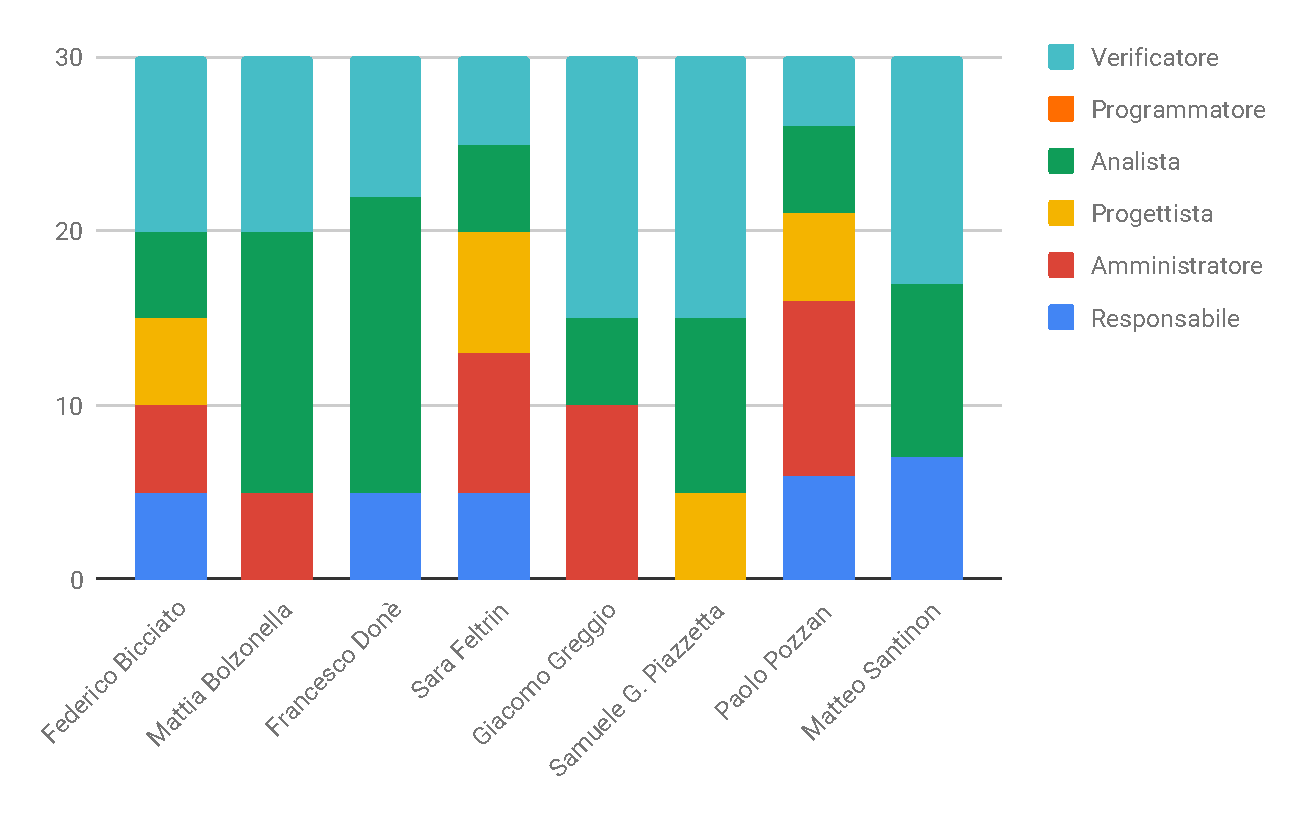
\includegraphics[width=0.9\textwidth]{res/images/istogramma_analisi.pdf}\\
				\caption{Istogramma della ripartizione di ore per ruolo in Analisi}
			\label{IstogrammaAnalisi}
\end{figure}


\subsubsection{Prospetto economico}
In questa fase il costo per ogni ruolo è il seguente:
\begin{table}[H]
				\centering\renewcommand{\arraystretch}{1.5}
				\arrayrulecolor{white}
                \begin{tabular}{c|c|c}
                               
                \rowcolorhead
                 {\colorhead \textbf{Ruolo}} &
                 {\colorhead \textbf{Ore}} & 
                 {\colorhead \textbf{Costo}} \\
				
                \rowcolorlight
                 {\colorbody Responsabile} & {\colorbody 23} & 
                 {\colorbody \EUR{690,00}}  
				\\
				
				\rowcolordark
                 {\colorbody Amministratore} & {\colorbody 19} & 
                 {\colorbody \EUR{380,00}}
				\\	
				
				\rowcolorlight
                 {\colorbody Analista} & {\colorbody 68} & 
                 {\colorbody \EUR{1.700,00}} 
				\\
				
				\rowcolordark
                 {\colorbody Progettista} & {\colorbody -} & 
                 {\colorbody -} 
				\\
				
				\rowcolorlight
                 {\colorbody Programmatore} & {\colorbody -} & 
                 {\colorbody -} 
				\\
				
				\rowcolordark
                 {\colorbody Verificatore} & {\colorbody 41} & 
                 {\colorbody \EUR{615,00}} 
				\\
				
				\rowcolorlight
                 {\colorbody \textbf{Totale}} & {\colorbody 151} & 
                 {\colorbody \EUR{3.385,00}} 
				\\
				
                

                \end{tabular}
                \caption{Prospetto dei costi per ruoli nel periodo di Analisi}
\end{table}

I dati ottenuti si possono riassumere nel seguente areogramma:
\begin{figure}[H] 
			\centering 
				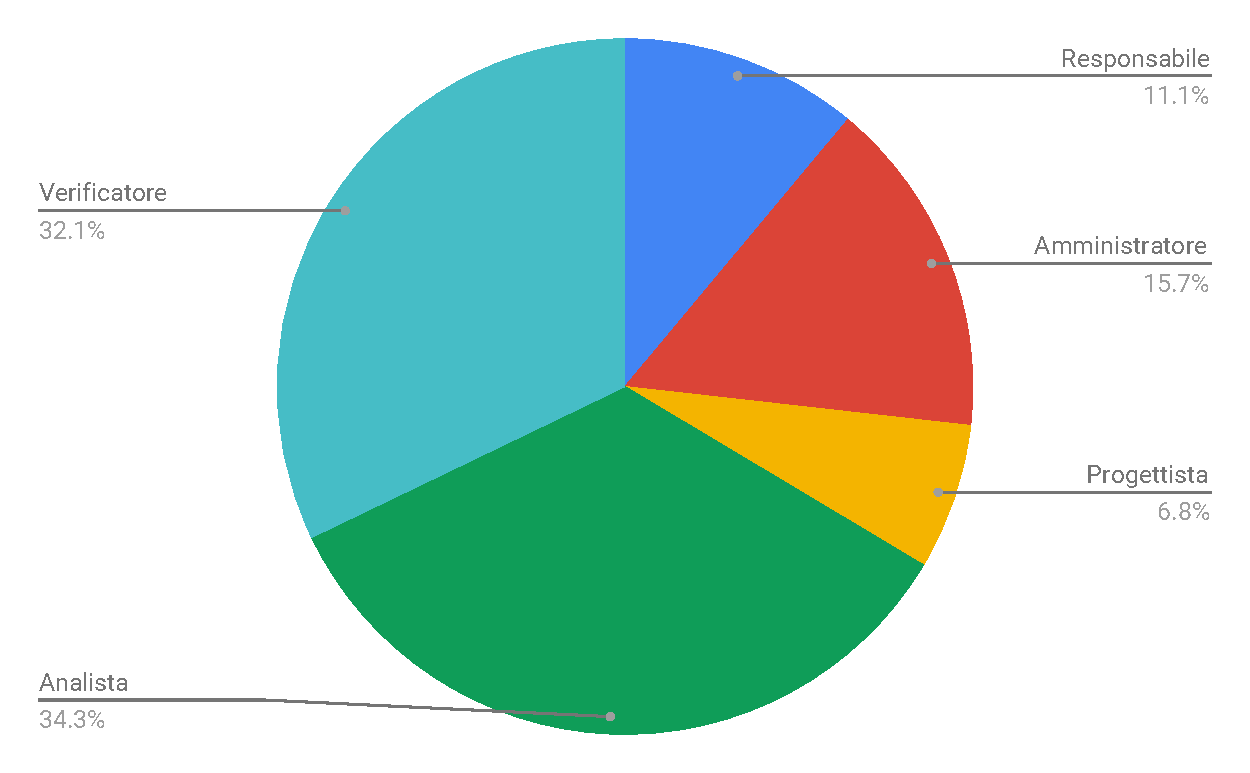
\includegraphics[width=0.7\textwidth]{res/images/areogramma_analisi.pdf}\\
				\caption{Areogramma della ripartizione di ore per ruolo in Analisi}
			\label{AreogrammaAnalisi}
\end{figure}

\subsection{Fase di Consolidamento dei requisiti}
\subsubsection{Prospetto orario}
Il periodo di Consolidamento dei requisiti vede la seguente distribuzione oraria:
\begin{table}[H]
				\centering\renewcommand{\arraystretch}{1.5}
				\arrayrulecolor{white}
                \begin{tabular}{c|c|c|c|c|c|c|c}
                               
                \rowcolorhead
                 {\colorhead \textbf{Nominativo}} &
                 {\colorhead \textbf{Re}} & 
                 {\colorhead \textbf{Am}} & 
                 {\colorhead\textbf{An}} & 
                 {\colorhead \textbf{Pt}} & 
                 {\colorhead\textbf{Pr}} & 
                 {\colorhead \textbf{Ve}} & 
                 {\colorhead \textbf{Ore totali} }\\
				
                \rowcolorlight
                 {\colorbody Federico Bicciato} & {\colorbody -} & 
                 {\colorbody -} & {\colorbody 5} & {\colorbody -} & 
                 {\colorbody -} & {\colorbody -} & {\colorbody 5} 
				\\
				
				\rowcolordark
                 {\colorbody Mattia Bolzonella} & {\colorbody -} & 
                 {\colorbody 5} & {\colorbody -} & {\colorbody -} & 
                 {\colorbody -} & {\colorbody -} & {\colorbody 5} 
				\\	
				
				\rowcolorlight
                 {\colorbody Francesco Donè} & {\colorbody -} & 
                 {\colorbody -} & {\colorbody 3} & {\colorbody -} & 
                 {\colorbody -} & {\colorbody 3} & {\colorbody 6} 
				\\
				
				\rowcolordark
                 {\colorbody Sara Feltrin} & {\colorbody 5} & 
                 {\colorbody -} & {\colorbody -} & {\colorbody -} & 
                 {\colorbody -} & {\colorbody -} & {\colorbody 5} 
				\\
                
                \rowcolorlight
                 {\colorbody Giacomo Greggio} & {\colorbody -} & 
                 {\colorbody -} & {\colorbody -} & {\colorbody -} & 
                 {\colorbody -} & {\colorbody 6} & {\colorbody 6} 
				\\
				
				\rowcolordark
                 {\colorbody Samuele Piazzetta} & {\colorbody -} & 
                 {\colorbody 3} & {\colorbody -} & {\colorbody -} & 
                 {\colorbody -} & {\colorbody 3} & {\colorbody 6} 
				\\	
				
				\rowcolorlight
                 {\colorbody Paolo Pozzan} & {\colorbody -} & 
                 {\colorbody -} & {\colorbody 4} & {\colorbody -} & 
                 {\colorbody -} & {\colorbody 2} & {\colorbody 6} 
				\\
				
				\rowcolordark
                 {\colorbody Matteo Santinon} & {\colorbody -} & 
                 {\colorbody -} & {\colorbody -} & {\colorbody -} & 
                 {\colorbody -} & {\colorbody 6} & {\colorbody 6} 
				\\
				
				\rowcolorlight
                 {\colorbody \textbf{Ore totali ruolo}} & {\colorbody 5} & 
                 {\colorbody 8} & {\colorbody 12} & {\colorbody -} & 
                 {\colorbody -} & {\colorbody 20} & { \colorbody 45} 
				\\

                \end{tabular}
                \caption{Distribuzione delle ore nel periodo di Consolidamento 
				dei requisiti}

\end{table}

I dati ottenuti si possono riassumere nel seguente istogramma:
\begin{figure}[H] 
			\centering 
				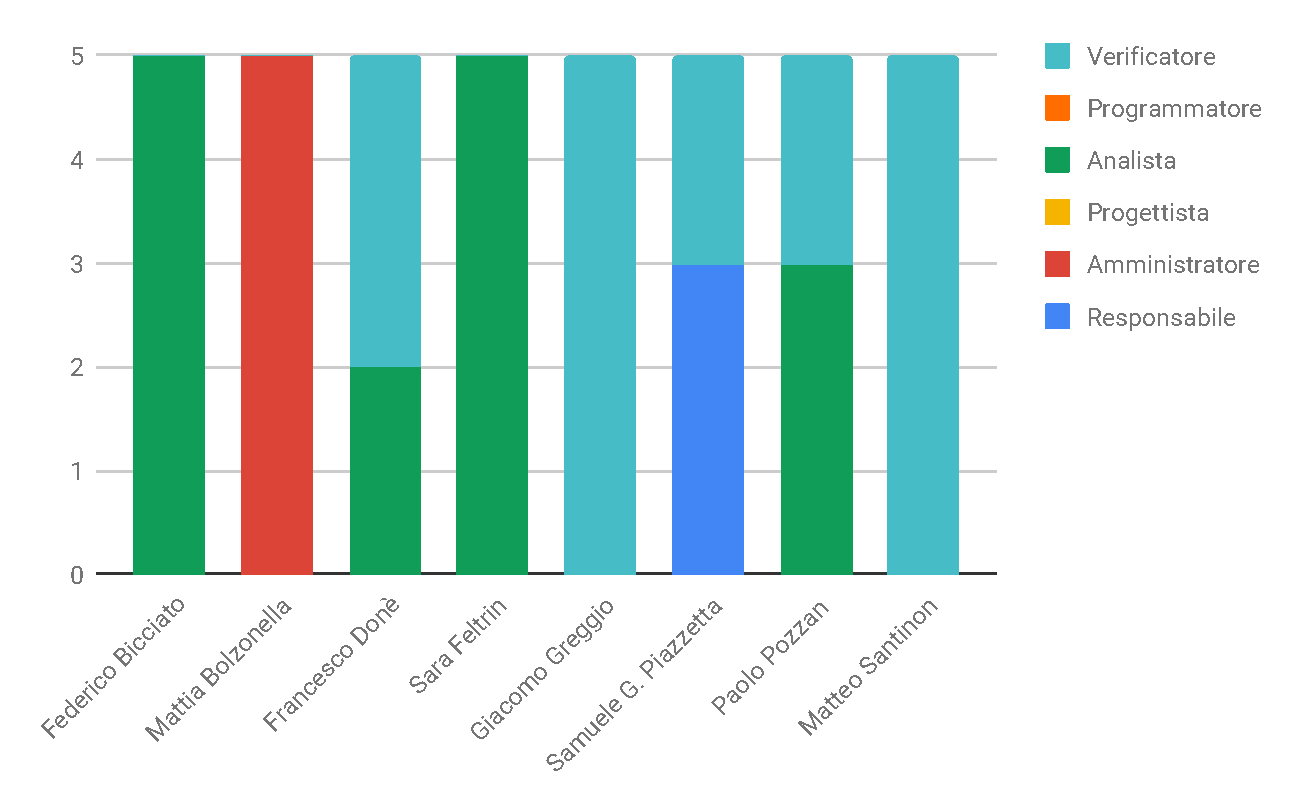
\includegraphics[width=0.9\textwidth]{res/images/istogramma_consolidamento.pdf}\\
				\caption{Istogramma della ripartizione di ore per ruolo in Consolidamento dei requisiti}
			\label{IstogrammaConsolidamento}
\end{figure}

\subsubsection{Prospetto economico}
In questa fase il costo per ogni ruolo è il seguente:
\begin{table}[H]
				\centering\renewcommand{\arraystretch}{1.5}
				\arrayrulecolor{white}
                \begin{tabular}{c|c|c}
                               
                \rowcolorhead
                 {\colorhead \textbf{Ruolo}} &
                 {\colorhead \textbf{Ore}} & 
                 {\colorhead \textbf{Costo}} \\
				
                \rowcolorlight
                 {\colorbody Responsabile} & {\colorbody 5} & 
                 {\colorbody \EUR{150,00}}  
				\\
				
				\rowcolordark
                 {\colorbody Amministratore} & {\colorbody 8} & 
                 {\colorbody \EUR{160,00}}
				\\	
				
				\rowcolorlight
                 {\colorbody Analista} & {\colorbody 12} & 
                 {\colorbody \EUR{300,00}} 
				\\
				
				\rowcolordark
                 {\colorbody Progettista} & {\colorbody -} & 
                 {\colorbody -} 
				\\
				
				\rowcolorlight
                 {\colorbody Programmatore} & {\colorbody -} & 
                 {\colorbody -} 
				\\
				
				\rowcolordark
                 {\colorbody Verificatore} & {\colorbody 20} & 
                 {\colorbody \EUR{300,00}} 
				\\
				
				\rowcolorlight
                 {\colorbody \textbf{Totale}} & {\colorbody 45} & 
                 {\colorbody \EUR{910,00}} 
				\\
                

                \end{tabular}
                \caption{Prospetto dei costi per ruoli nel periodo di 
				Consolidamento dei requisiti}

\end{table}

I dati ottenuti si possono riassumere nel seguente areogramma:
\begin{figure}[H] 
			\centering 
				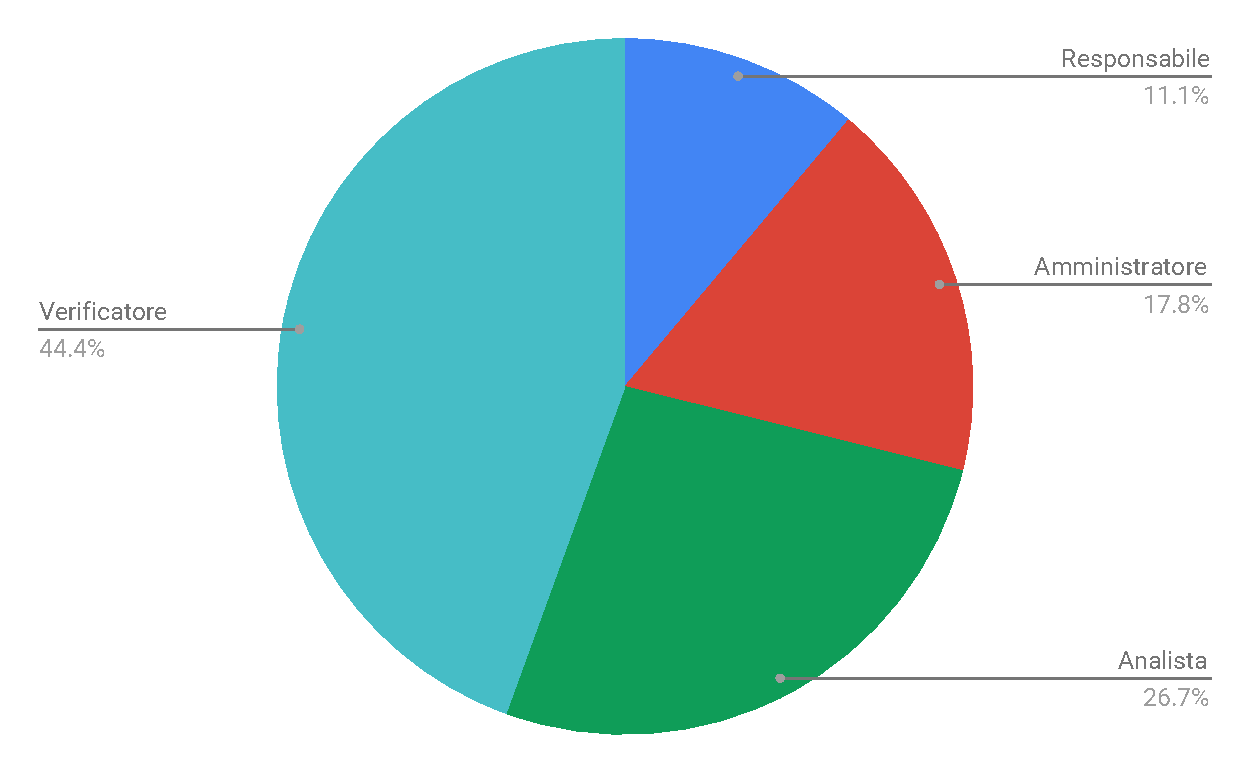
\includegraphics[width=0.7\textwidth]{res/images/areogramma_consolidamento.pdf}\\
				\caption{Areogramma della ripartizione di ore per ruolo in Consolidamento dei requisiti}
			\label{AreogrammaConsolidaemnto}
\end{figure}

\subsection{Fase di Progettazione architetturale}
\subsubsection{Prospetto orario}
Nella fase di Progettazione architetturale la distribuzione oraria è la seguente:
\begin{table}[H]
				\centering\renewcommand{\arraystretch}{1.5}
				\arrayrulecolor{white}
                \begin{tabular}{c|c|c|c|c|c|c|c}
                               
                \rowcolorhead
                 {\colorhead \textbf{Nominativo}} &
                 {\colorhead \textbf{Re}} & 
                 {\colorhead \textbf{Am}} & 
                 {\colorhead\textbf{An}} & 
                 {\colorhead \textbf{Pt}} & 
                 {\colorhead\textbf{Pr}} & 
                 {\colorhead \textbf{Ve}} & 
                 {\colorhead \textbf{Ore totali} }\\
				
                \rowcolorlight
                 {\colorbody Federico Bicciato} & {\colorbody -} & 
                 {\colorbody -} & {\colorbody 12} & {\colorbody -} & 
                 {\colorbody -} & {\colorbody 12} & {\colorbody 24} 
				\\
				
				\rowcolordark
                 {\colorbody Mattia Bolzonella} & {\colorbody 6} & 
                 {\colorbody -} & {\colorbody -} & {\colorbody 8} & 
                 {\colorbody -} & {\colorbody 10} & {\colorbody 24} 
				\\	
				
				\rowcolorlight
                 {\colorbody Francesco Donè} & {\colorbody -} & 
                 {\colorbody -} & {\colorbody -} & {\colorbody 12} & 
                 {\colorbody -} & {\colorbody 12} & {\colorbody 24} 
				\\
				
				\rowcolordark
                 {\colorbody Sara Feltrin} & {\colorbody -} & 
                 {\colorbody -} & {\colorbody -} & {\colorbody 14} & 
                 {\colorbody -} & {\colorbody 10} & {\colorbody 24} 
				\\
                
                \rowcolorlight
                 {\colorbody Giacomo Greggio} & {\colorbody -} & 
                 {\colorbody -} & {\colorbody -} & {\colorbody 13} & 
                 {\colorbody -} & {\colorbody 10} & {\colorbody 23} 
				\\
				
				\rowcolordark
                 {\colorbody Samuele Piazzetta} & {\colorbody 2} & 
                 {\colorbody 3} & {\colorbody -} & {\colorbody 18} & 
                 {\colorbody -} & {\colorbody -} & {\colorbody 24} 
				\\	
				
				\rowcolorlight
                 {\colorbody Paolo Pozzan} & {\colorbody -} & 
                 {\colorbody -} & {\colorbody -} & {\colorbody 18} & 
                 {\colorbody -} & {\colorbody 6} & {\colorbody 24} 
				\\
				
				\rowcolordark
                 {\colorbody Matteo Santinon} & {\colorbody -} & 
                 {\colorbody 7} & {\colorbody 6} & {\colorbody 11} & 
                 {\colorbody -} & {\colorbody -} & {\colorbody 24} 
				\\
				
				\rowcolorlight
                 {\colorbody \textbf{Ore totali ruolo}} & {\colorbody 8} & 
                 {\colorbody 10} & {\colorbody 18} & {\colorbody 94} & 
                 {\colorbody -} & {\colorbody 60} & {\colorbody 190} 
				\\

                \end{tabular}
                \caption{Distribuzione delle ore nel periodo di Progettazione 
				architetturale}

\end{table}

Una rappresentazione visiva della suddivisione oraria viene data dal seguente grafico:
\begin{figure}[H] 
			\centering 
				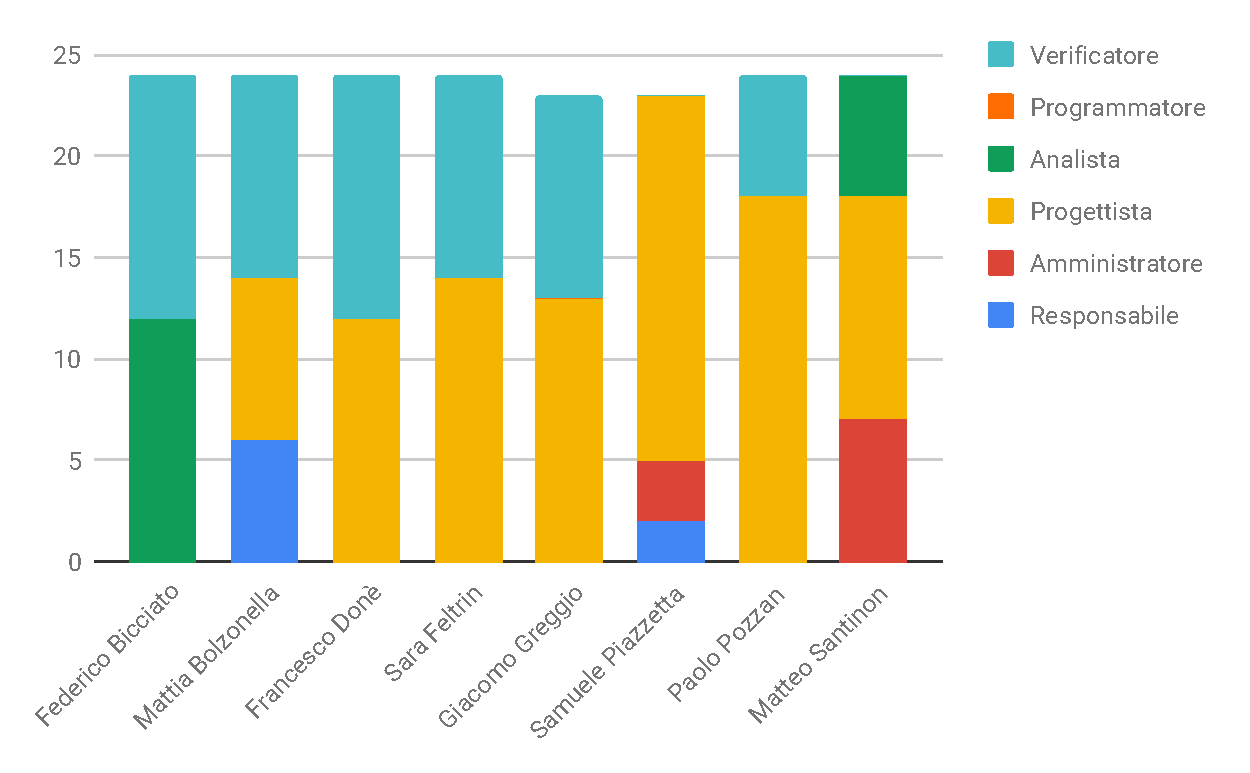
\includegraphics[width=0.9\textwidth]{res/images/istogramma_architetturale.pdf}\\
				\caption{Istogramma della ripartizione di ore per ruolo in Progettazione architetturale}
			\label{IstogrammaArchitetturale}
\end{figure}

\subsubsection{Prospetto economico}
In questa fase il costo per ogni ruolo è il seguente:
\begin{table}[H]
				\centering\renewcommand{\arraystretch}{1.5}
				\arrayrulecolor{white}
                \begin{tabular}{c|c|c}
                               
                \rowcolorhead
                 {\colorhead \textbf{Ruolo}} &
                 {\colorhead \textbf{Ore}} & 
                 {\colorhead \textbf{Costo}} \\
				
                \rowcolorlight
                 {\colorbody Responsabile} & {\colorbody 8} & 
                 {\colorbody \EUR{240,00}}  
				\\
				
				\rowcolordark
                 {\colorbody Amministratore} & {\colorbody 10} & 
                 {\colorbody \EUR{200,00}}
				\\	
				
				\rowcolorlight
                 {\colorbody Analista} & {\colorbody 18} & 
                 {\colorbody \EUR{450,00}} 
				\\
				
				\rowcolordark
                 {\colorbody Progettista} & {\colorbody 94} & 
                 {\colorbody \EUR{2.068,00}} 
				\\
				
				\rowcolorlight
                 {\colorbody Programmatore} & {\colorbody -} & 
                 {\colorbody -} 
				\\
				
				\rowcolordark
                 {\colorbody Verificatore} & {\colorbody 60} & 
                 {\colorbody \EUR{900,00}} 
				\\
				
				\rowcolorlight
                 {\colorbody \textbf{Totale}} & {\colorbody 190} & 
                 {\colorbody \EUR{3.858,00}} 
				\\
                

                \end{tabular}
                \caption{Prospetto dei costi per ruoli nel periodo di 
				Progettazione architetturale}

\end{table}
I dati ottenuti si possono riassumere nel seguente areogramma:
\begin{figure}[H] 
			\centering 
				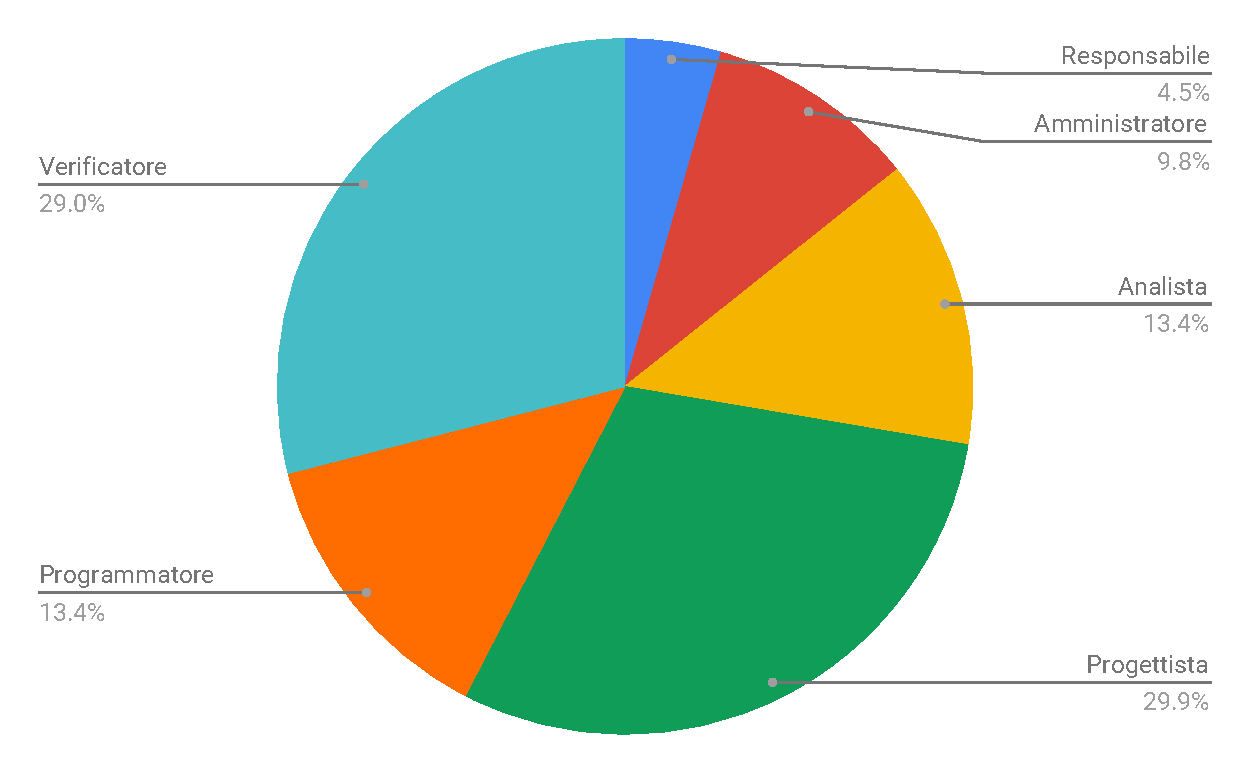
\includegraphics[width=0.7\textwidth]{res/images/areogramma_architetturale.pdf}\\
				\caption{Areogramma della ripartizione di ore per ruolo in Progettazione architetturale}
			\label{AreogrammaArchitetturale}
\end{figure}

\subsection{Fase di Progettazione di dettaglio e codifica}
\subsubsection{Prospetto orario}
Nella fase di Progettazione di dettaglio e codifica la distribuzione oraria è la seguente:
\begin{table}[H]
				\centering\renewcommand{\arraystretch}{1.5}
				\arrayrulecolor{white}
                \begin{tabular}{c|c|c|c|c|c|c|c}
                               
                \rowcolorhead
                 {\colorhead \textbf{Nominativo}} &
                 {\colorhead \textbf{Re}} & 
                 {\colorhead \textbf{Am}} & 
                 {\colorhead\textbf{An}} & 
                 {\colorhead \textbf{Pt}} & 
                 {\colorhead\textbf{Pr}} & 
                 {\colorhead \textbf{Ve}} & 
                 {\colorhead \textbf{Ore totali} }\\
				
                \rowcolorlight
                 {\colorbody Federico Bicciato} & {\colorbody -} & 
                 {\colorbody -} & {\colorbody -} & {\colorbody 16} & 
                 {\colorbody 17} & {\colorbody 9} & {\colorbody 42} 
				\\
				
				\rowcolordark
                 {\colorbody Mattia Bolzonella} & {\colorbody -} & 
                 {\colorbody -} & {\colorbody -} & {\colorbody 11} & 
                 {\colorbody 18} & {\colorbody 13} & {\colorbody 42} 
				\\	
				
				\rowcolorlight
                 {\colorbody Francesco Donè} & {\colorbody -} & 
                 {\colorbody -} & {\colorbody -} & {\colorbody 15} & 
                 {\colorbody 17} & {\colorbody 9} & {\colorbody 41} 
				\\
				
				\rowcolordark
                 {\colorbody Sara Feltrin} & {\colorbody -} & 
                 {\colorbody -} & {\colorbody 4} & {\colorbody 12} & 
                 {\colorbody 17} & {\colorbody 9} & { \colorbody 42} 
				\\
                
                \rowcolorlight
                 {\colorbody Giacomo Greggio} & {\colorbody -} & 
                 {\colorbody 8} & {\colorbody -} & {\colorbody 12} & 
                 {\colorbody 10} & {\colorbody 12} & {\colorbody 42} 
				\\
				
				\rowcolordark
                 {\colorbody Samuele Piazzetta} & {\colorbody 6} & 
                 {\colorbody -} & {\colorbody -} & {\colorbody 13} & 
                 {\colorbody 8} & {\colorbody 15} & {\colorbody 42} 
				\\	
				
				\rowcolorlight
                 {\colorbody Paolo Pozzan} & {\colorbody 8} & 
                 {\colorbody -} & {\colorbody -} & {\colorbody 11} & 
                 {\colorbody 18} & {\colorbody 4} & {\colorbody 41} 
				\\
				
				\rowcolordark
                 {\colorbody Matteo Santinon} & {\colorbody -} & 
                 {\colorbody -} & {\colorbody -} & {\colorbody 18} & 
                 {\colorbody 16} & {\colorbody 8} & {\colorbody 42} 
				\\
				
				\rowcolorlight
                 {\colorbody \textbf{Ore totali ruolo}} & {\colorbody 14} & 
                 {\colorbody 8} & {\colorbody 4} & {\colorbody 108} & 
                 {\colorbody 121} & {\colorbody 79} & {\colorbody 334} 
				\\

                \end{tabular}
                \caption{Distribuzione delle ore nel periodo di Progettazione di 
				dettaglio e codifica}

\end{table}

Una rappresentazione visiva della suddivisione oraria viene data dal seguente grafico:
\begin{figure}[H] 
			\centering 
				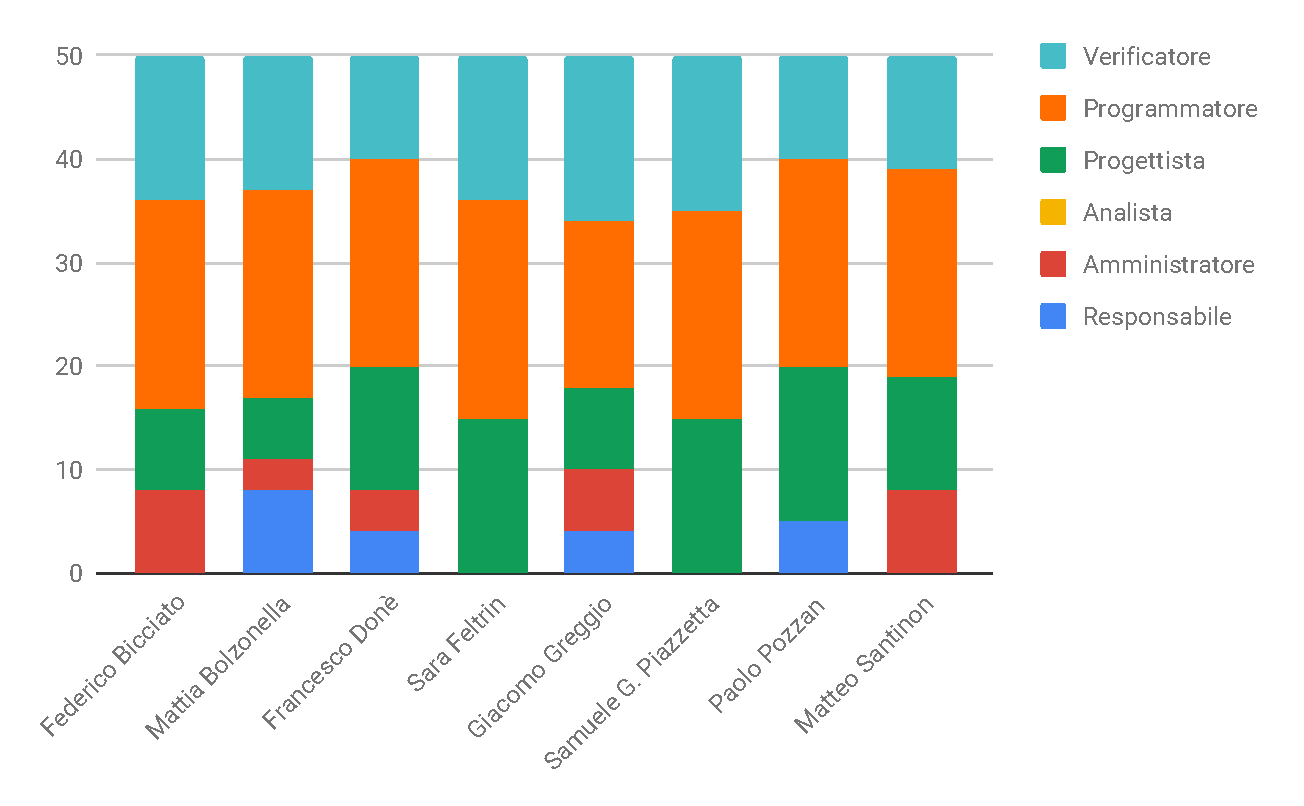
\includegraphics[width=0.9\textwidth]{res/images/istogramma_dettaglio.pdf}\\
				\caption{Istogramma della ripartizione di ore per ruolo in Progettazione di dettaglio e codifica}
			\label{IstogrammaDettaglio}
\end{figure}

\subsubsection{Prospetto economico}
In questa fase il costo per ogni ruolo è il seguente:
\begin{table}[H]
				\centering\renewcommand{\arraystretch}{1.5}
				\arrayrulecolor{white}
                \begin{tabular}{c|c|c}
                               
                \rowcolorhead
                 {\colorhead \textbf{Ruolo}} &
                 {\colorhead \textbf{Ore}} & 
                 {\colorhead \textbf{Costo}} \\
				
                \rowcolorlight
                 {\colorbody Responsabile} & {\colorbody 14} & 
                 {\colorbody \EUR{420,00}}  
				\\
				
				\rowcolordark
                 {\colorbody Amministratore} & {\colorbody 8} & 
                 {\colorbody \EUR{160,00}}
				\\	
				
				\rowcolorlight
                 {\colorbody Analista} & {\colorbody 4} & 
                 {\colorbody \EUR{100,00}} 
				\\
				
				\rowcolordark
                 {\colorbody Progettista} & {\colorbody 108} & 
                 {\colorbody \EUR{2.376,00}} 
				\\
				
				\rowcolorlight
                 {\colorbody Programmatore} & {\colorbody 121} & 
                 {\colorbody \EUR{1.815,00}} 
				\\
				
				\rowcolordark
                 {\colorbody Verificatore} & {\colorbody 79} & 
                 {\colorbody \EUR{1.185,00}} 
				\\
				
				\rowcolorlight
                 {\colorbody \textbf{Totale}} & {\colorbody 334} & 
                 {\colorbody \EUR{6.056,00}} 
				\\
                

                \end{tabular}
                \caption{Prospetto dei costi per ruoli nel periodo di 
				Progettazione di dettaglio e codifica}

\end{table}

I dati ottenuti si possono riassumere nel seguente areogramma:
\begin{figure}[H] 
			\centering 
				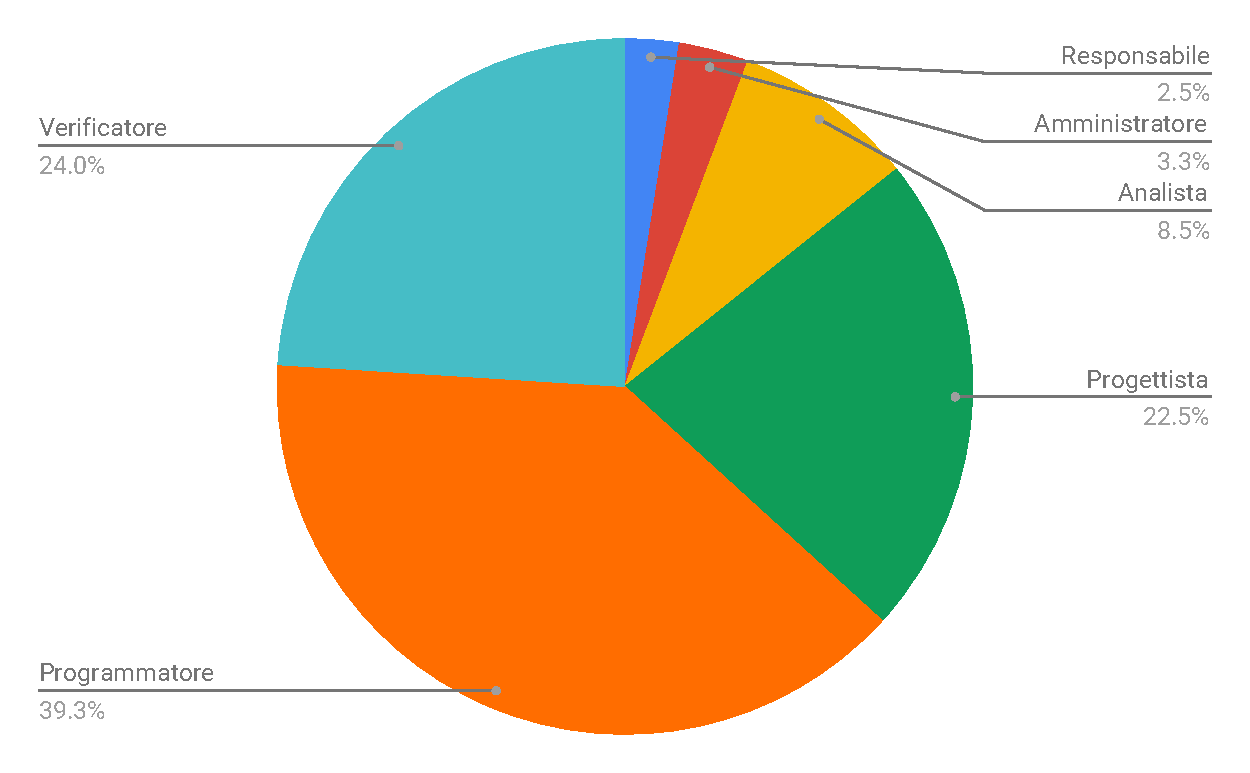
\includegraphics[width=0.7\textwidth]{res/images/areogramma_dettaglio.pdf}\\
				\caption{Areogramma della ripartizione di ore per ruolo in Progettazione di dettaglio e codifica}
			\label{AreogrammaDettaglio}
\end{figure}


\subsection{Fase di Validazione e collaudo}
\subsubsection{Prospetto orario}
Nella fase di progettazione di Validazione e collaudo la distribuzione oraria è la seguente:
\begin{table}[H]
				\centering\renewcommand{\arraystretch}{1.5}
				\arrayrulecolor{white}
                \begin{tabular}{c|c|c|c|c|c|c|c}
                               
                \rowcolorhead
                 {\colorhead \textbf{Nominativo}} &
                 {\colorhead \textbf{Re}} & 
                 {\colorhead \textbf{Am}} & 
                 {\colorhead\textbf{An}} & 
                 {\colorhead \textbf{Pt}} & 
                 {\colorhead\textbf{Pr}} & 
                 {\colorhead \textbf{Ve}} & 
                 {\colorhead \textbf{Ore totali} }\\
				
                \rowcolorlight
                 {\colorbody Federico Bicciato} & {\colorbody -} & 
                 {\colorbody -} & {\colorbody -} & {\colorbody 9} & 
                 {\colorbody -} & {\colorbody 6} & {\colorbody 15} 
				\\
				
				\rowcolordark
                 {\colorbody Mattia Bolzonella} & {\colorbody -} & 
                 {\colorbody 4} & {\colorbody -} & {\colorbody 11} & 
                 {\colorbody -} & {\colorbody -} & {\colorbody 15} 
				\\	
				
				\rowcolorlight
                 {\colorbody Francesco Donè} & {\colorbody 3} & 
                 {\colorbody 5} & {\colorbody -} & {\colorbody -} & 
                 {\colorbody 7} & {\colorbody -} & {\colorbody 15} 
				\\
				
				\rowcolordark
                 {\colorbody Sara Feltrin} & {\colorbody 4} & 
                 {\colorbody -} & {\colorbody -} & {\colorbody -} & 
                 {\colorbody -} & {\colorbody 11} & {\colorbody 15} 
				\\
                
                \rowcolorlight
                 {\colorbody Giacomo Greggio} & {\colorbody -} & 
                 {\colorbody -} & {\colorbody -} & {\colorbody -} & 
                 {\colorbody 7} & {\colorbody 8} & {\colorbody 15} 
				\\
				
				\rowcolordark
                 {\colorbody Samuele Piazzetta} & {\colorbody -} & 
                 {\colorbody -} & {\colorbody -} & {\colorbody -} & 
                 {\colorbody 9} & {\colorbody 6} & {\colorbody 15} 
				\\	
				
				\rowcolorlight
                 {\colorbody Paolo Pozzan} & {\colorbody -} & 
                 {\colorbody 3} & {\colorbody -} & {\colorbody -} & 
                 {\colorbody -} & {\colorbody 12} & {\colorbody 15} 
				\\
				
				\rowcolordark
                 {\colorbody Matteo Santinon} & {\colorbody 3} & 
                 {\colorbody -} & {\colorbody -} & {\colorbody -} & 
                 {\colorbody -} & {\colorbody 12} & {\colorbody 15} 
				\\
				
				\rowcolorlight
                 {\colorbody \textbf{Ore totali ruolo}} & {\colorbody 10} & 
                 {\colorbody 12} & {\colorbody 20} & {\colorbody -} & 
                 {\colorbody 23} & {\colorbody 55} & {\colorbody 120} 
				\\

                \end{tabular}
                \caption{Distribuzione delle ore nel periodo di Validazione e 
				collaudo}
\end{table}

Una rappresentazione visiva della suddivisione oraria viene data dal seguente grafico:
\begin{figure}[H] 
			\centering 
				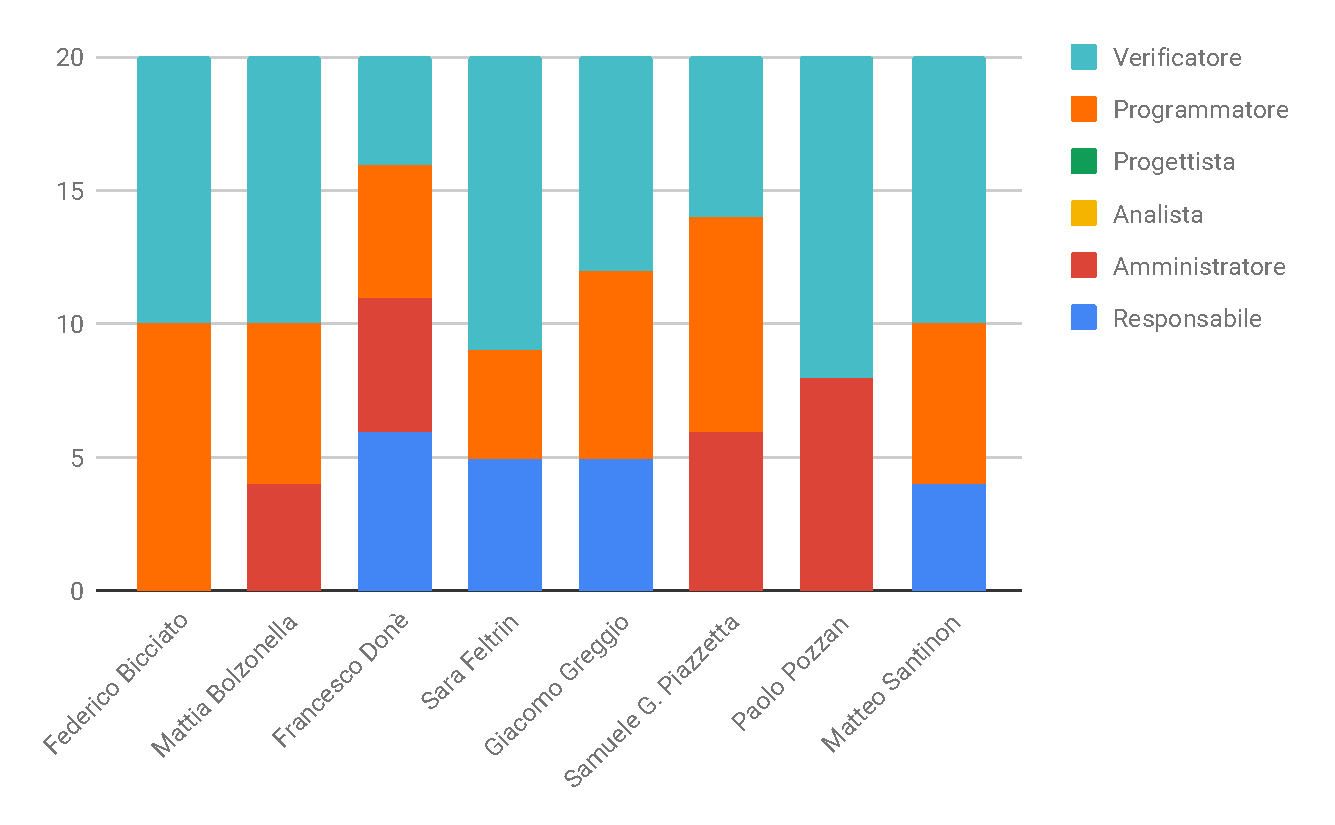
\includegraphics[width=0.9\textwidth]{res/images/istogramma_validazione.pdf}\\
				\caption{Istogramma della ripartizione di ore per ruolo in Validazione e collaudo}
			\label{IstogrammaValidazione}
\end{figure}

\subsubsection{Prospetto economico}
In questa fase il costo per ogni ruolo è il seguente:
\begin{table}[H]
				\centering\renewcommand{\arraystretch}{1.5}
				\arrayrulecolor{white}
                \begin{tabular}{c|c|c}
                               
                \rowcolorhead
                 {\colorhead \textbf{Ruolo}} &
                 {\colorhead \textbf{Ore}} & 
                 {\colorhead \textbf{Costo}} \\
				
                \rowcolorlight
                 {\colorbody Responsabile} & {\colorbody 10} & 
                 {\colorbody \EUR{300,00}}  
				\\
				
				\rowcolordark
                 {\colorbody Amministratore} & {\colorbody 12} & 
                 {\colorbody \EUR{240,00}}
				\\	
				
				\rowcolorlight
                 {\colorbody Analista} & {\colorbody 20} & 
                 {\colorbody \EUR{440,00}} 
				\\
				
				\rowcolordark
                 {\colorbody Progettista} & {\colorbody -} & 
                 {\colorbody -} 
				\\
				
				\rowcolorlight
                 {\colorbody Programmatore} & {\colorbody 23} & 
                 {\colorbody \EUR{345,00}} 
				\\
				
				\rowcolordark
                 {\colorbody Verificatore} & {\colorbody 55} & 
                 {\colorbody \EUR{825,00}} 
				\\
				
				\rowcolorlight
                 {\colorbody \textbf{Totale}} & {\colorbody 120} & 
                 {\colorbody \EUR{2.150,00}} 
				\\
                

                \end{tabular}
                \caption{Prospetto dei costi per ruoli nel periodo di 
				Validazione e collaudo}

\end{table}

I dati ottenuti si possono riassumere nel seguente areogramma:
\begin{figure}[H] 
			\centering 
				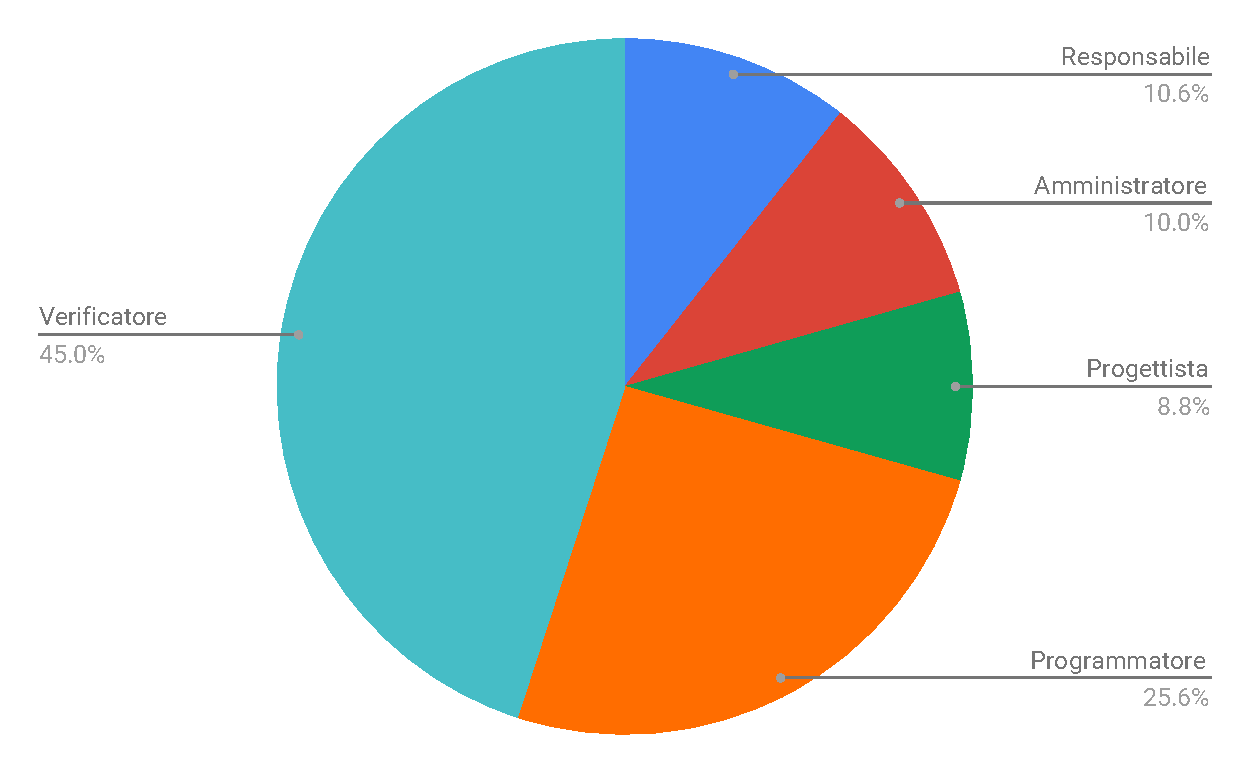
\includegraphics[width=0.7\textwidth]{res/images/areogramma_validazione.pdf}\\
				\caption{Areogramma della ripartizione di ore per ruolo in Validazione e collaudo}
			\label{AreogrammaValidazione}
\end{figure}


\subsection{Riepilogo}
\subsubsection{Ore totali}
\paragraph{Suddivisione del lavoro}\mbox{}\\
Vengono riportate il totale delle ore del progetto in cui sono presenti le ore di investimento e le ore rendicontate a carico del committente:
\begin{table}[H]
				\centering\renewcommand{\arraystretch}{1.5}
				\arrayrulecolor{white}
                \begin{tabular}{c|c|c|c|c|c|c|c}
                               
                \rowcolorhead
                 {\colorhead \textbf{Nominativo}} &
                 {\colorhead \textbf{Re}} & 
                 {\colorhead \textbf{Am}} & 
                 {\colorhead\textbf{An}} & 
                 {\colorhead \textbf{Pt}} & 
                 {\colorhead\textbf{Pr}} & 
                 {\colorhead \textbf{Ve}} & 
                 {\colorhead \textbf{Ore totali} }\\
				
                \rowcolorlight
                 {\colorbody Federico Bicciato} & {\colorbody 6} & 
                 {\colorbody 9} & {\colorbody 17} & {\colorbody 25} & 
                 {\colorbody 17} & {\colorbody 31} & {\colorbody 105} 
				\\
				
				\rowcolordark
                 {\colorbody Mattia Bolzonella} & {\colorbody 6} & 
                 {\colorbody 9} & {\colorbody 12} & {\colorbody 30} & 
                 {\colorbody 18} & {\colorbody 30} & {\colorbody 105} 
				\\	
				
				\rowcolorlight
                 {\colorbody Francesco Donè} & {\colorbody 9} & 
                 {\colorbody 5} & {\colorbody 11} & {\colorbody 27} & 
                 {\colorbody 24} & {\colorbody 29} & {\colorbody 105} 
				\\
				
				\rowcolordark
                 {\colorbody Sara Feltrin} & {\colorbody 9} & 
                 {\colorbody 5} & {\colorbody 15} & {\colorbody 26} & 
                 {\colorbody 17} & {\colorbody 34} & {\colorbody 105} 
				\\
                
                \rowcolorlight
                 {\colorbody Giacomo Greggio} & {\colorbody 6} & 
                 {\colorbody 8} & {\colorbody 10} & {\colorbody 25} & 
                 {\colorbody 17} & {\colorbody 39} & {\colorbody 105} 
				\\
				
				\rowcolordark
                 {\colorbody Samuele Piazzetta} & {\colorbody 8} & 
                 {\colorbody 6} & {\colorbody 14} & {\colorbody 31} & 
                 {\colorbody 17} & {\colorbody 29} & {\colorbody 105} 
				\\	
				
				\rowcolorlight
                 {\colorbody Paolo Pozzan} & {\colorbody 8} & 
                 {\colorbody 8} & {\colorbody 10} & {\colorbody 29} & 
                 {\colorbody 18} & {\colorbody 32} & {\colorbody 105} 
				\\
				
				\rowcolordark
                 {\colorbody Matteo Santinon} & {\colorbody 8} & 
                 {\colorbody 7} & {\colorbody 14} & {\colorbody 29} & 
                 {\colorbody 16} & {\colorbody 31} & {\colorbody 105} 
				\\
				
				\rowcolorlight
                 {\colorbody \textbf{Ore totali ruolo}} & {\colorbody 60} & 
                 {\colorbody 57} & {\colorbody 102} & {\colorbody 222} & 
                 {\colorbody144 } & {\colorbody 255} & {\colorbody 840} 
				\\

                \end{tabular}
                \caption{Distribuzione delle ore totali di investimento e rendicontate}

\end{table}

Una rappresentazione visiva della suddivisione oraria viene data dal seguente grafico:
\begin{figure}[H] 
			\centering 
				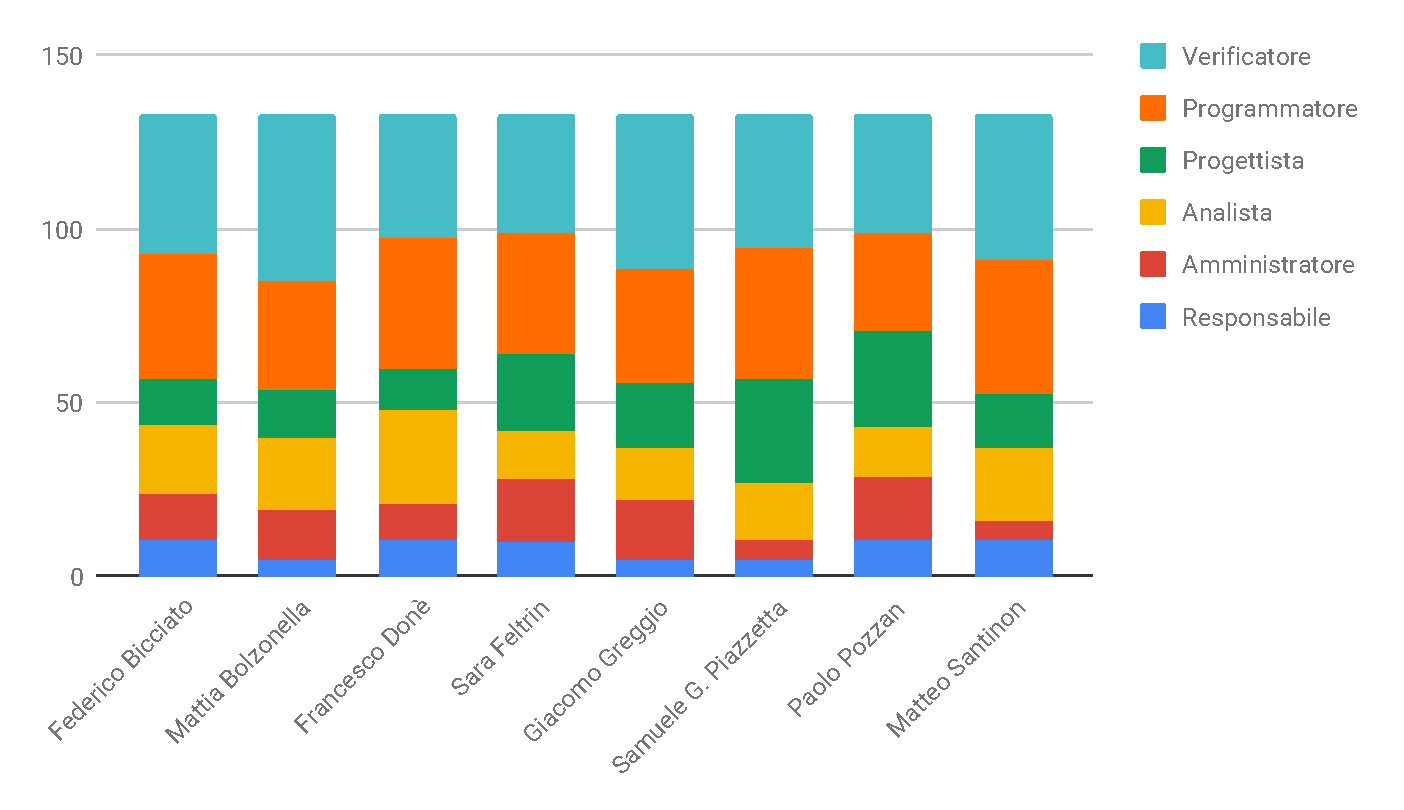
\includegraphics[width=0.9\textwidth]{res/images/istogramma_riepilogo.pdf}\\
				\caption{Istogramma della ripartizione di ore totali di investimento e rendicontate}
			\label{IstogrammaRiepilogo}
\end{figure}

\paragraph{Prospetto economico}\mbox{}\\
In questa fase il costo per ogni ruolo è il seguente:
\begin{table}[H]
				\centering\renewcommand{\arraystretch}{1.5}
				\arrayrulecolor{white}
                \begin{tabular}{c|c|c}
                               
                \rowcolorhead
                 {\colorhead \textbf{Ruolo}} &
                 {\colorhead \textbf{Ore}} & 
                 {\colorhead \textbf{Costo}} \\
				
                \rowcolorlight
                 {\colorbody Responsabile} & {\colorbody 60} & 
                 {\colorbody \EUR{1.800,00}}  
				\\
				
				\rowcolordark
                 {\colorbody Amministratore} & {\colorbody 57} & 
                 {\colorbody \EUR{1.140,00}}
				\\	
				
				\rowcolorlight
                 {\colorbody Analista} & {\colorbody 102} & 
                 {\colorbody \EUR{2.550,00}} 
				\\
				
				\rowcolordark
                 {\colorbody Progettista} & {\colorbody 222} & 
                 {\colorbody \EUR{4.884,00}} 
				\\
				
				\rowcolorlight
                 {\colorbody Programmatore} & {\colorbody 144} & 
                 {\colorbody \EUR{2.160,00}} 
				\\
				
				\rowcolordark
                 {\colorbody Verificatore} & {\colorbody 255} & 
                 {\colorbody \EUR{3.825,00}} 
				\\
				
				\rowcolorlight
                 {\colorbody \textbf{Totale}} & {\colorbody 840} & 
                 {\colorbody \EUR{16.359,00}} 
				\\
                

                \end{tabular}
                \caption{Prospetto dei costi totale delle ore di investimento e rendicontate}

\end{table}

I dati ottenuti si possono riassumere nel seguente diagramma:
\begin{figure}[H] 
			\centering 
				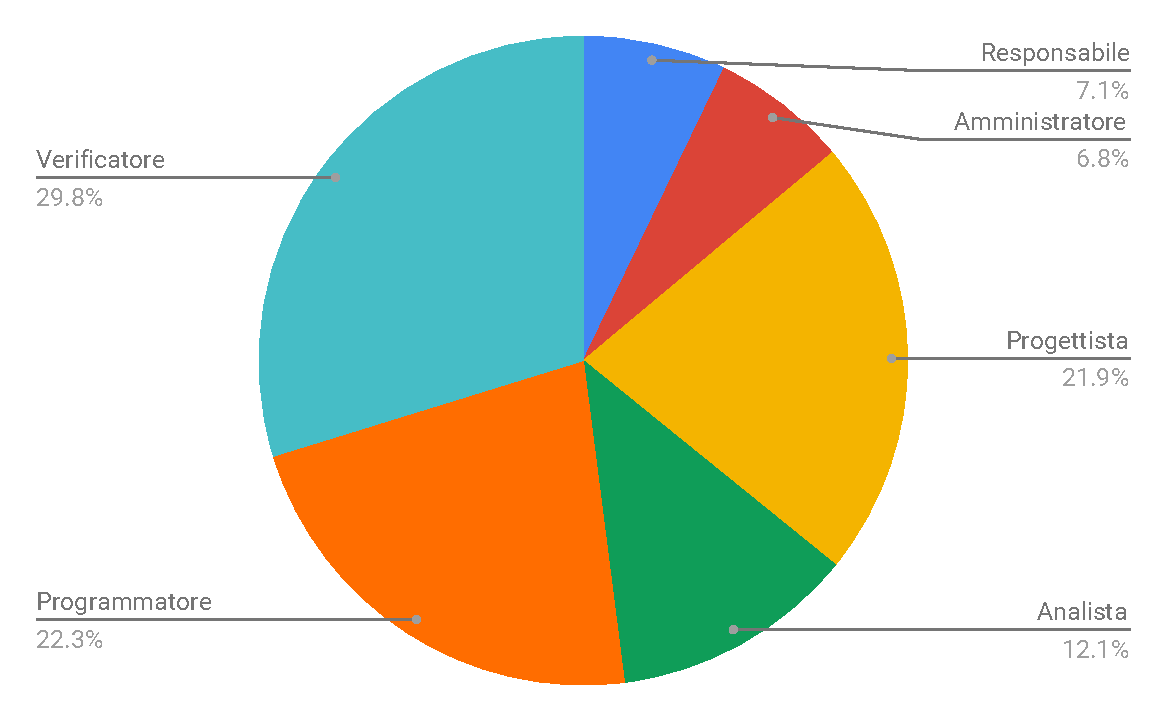
\includegraphics[width=0.7\textwidth]{res/images/areogramma_riepilogo.pdf}\\
				\caption{Areogramma dei costi totale delle ore di investimento e rendicontate}
			\label{AreogrammaRiepilogoRuoli}
\end{figure}


\subsubsection{Ore rendicontate}
\paragraph{Suddivisione del lavoro}\mbox{}\\
\linebreak
Le ore rendicontate sono riassunte nella seguente tabella:
\begin{table}[H]
				\centering\renewcommand{\arraystretch}{1.5}
				\arrayrulecolor{white}
                \begin{tabular}{c|c|c|c|c|c|c|c}
                               
                \rowcolorhead
                 {\colorhead \textbf{Nominativo}} &
                 {\colorhead \textbf{Re}} & 
                 {\colorhead \textbf{Am}} & 
                 {\colorhead\textbf{An}} & 
                 {\colorhead \textbf{Pt}} & 
                 {\colorhead\textbf{Pr}} & 
                 {\colorhead \textbf{Ve}} & 
                 {\colorhead \textbf{Ore totali} }\\
				
                \rowcolorlight
                 {\colorbody Federico Bicciato} & {\colorbody 6} & 
                 {\colorbody 4} & {\colorbody 12} & {\colorbody 22} & 
                 {\colorbody 17} & {\colorbody 30} & {\colorbody 91} 
				\\
				
				\rowcolordark
                 {\colorbody Mattia Bolzonella} & {\colorbody 4} & 
                 {\colorbody 6} & {\colorbody 10} & {\colorbody 30} & 
                 {\colorbody 18} & {\colorbody 23} & {\colorbody 91} 
				\\	
				
				\rowcolorlight
                 {\colorbody Francesco Donè} & {\colorbody 9} & 
                 {\colorbody 5} & {\colorbody 10} & {\colorbody 23} & 
                 {\colorbody 23} & {\colorbody 21} & {\colorbody 91} 
				\\
				
				\rowcolordark
                 {\colorbody Sara Feltrin} & {\colorbody 5} & 
                 {\colorbody 5} & {\colorbody 14} & {\colorbody 26} & 
                 {\colorbody 14} & {\colorbody 27} & {\colorbody 91} 
				\\
                
                \rowcolorlight
                 {\colorbody Giacomo Greggio} & {\colorbody 4} & 
                 {\colorbody 8} & {\colorbody 10} & {\colorbody 23} & 
                 {\colorbody 12} & {\colorbody 34} & {\colorbody 91} 
				\\
				
				\rowcolordark
                 {\colorbody Samuele Piazzetta} & {\colorbody 6} & 
                 {\colorbody 6} & {\colorbody 12} & {\colorbody 28} & 
                 {\colorbody 13} & {\colorbody 26} & {\colorbody 91} 
				\\	
				
				\rowcolorlight
                 {\colorbody Paolo Pozzan} & {\colorbody 8} & 
                 {\colorbody 5} & {\colorbody 10} & {\colorbody 25} & 
                 {\colorbody 16} & {\colorbody 27} & {\colorbody 91} 
				\\
				
				\rowcolordark
                 {\colorbody Matteo Santinon} & {\colorbody 5} & 
                 {\colorbody 7} & {\colorbody 14} & {\colorbody 27} & 
                 {\colorbody 14} & {\colorbody 24} & {\colorbody 91} 
				\\
				
				\rowcolorlight
                 {\colorbody \textbf{Ore totali ruolo}} & {\colorbody 47} & 
                 {\colorbody 49} & {\colorbody 92} & {\colorbody 204} & 
                 {\colorbody 127} & {\colorbody 212} & {\colorbody 728} 
				\\

                \end{tabular}
                \caption{Distribuzione delle ore rendicontate}

\end{table}

\begin{figure}[H] 
			\centering 
				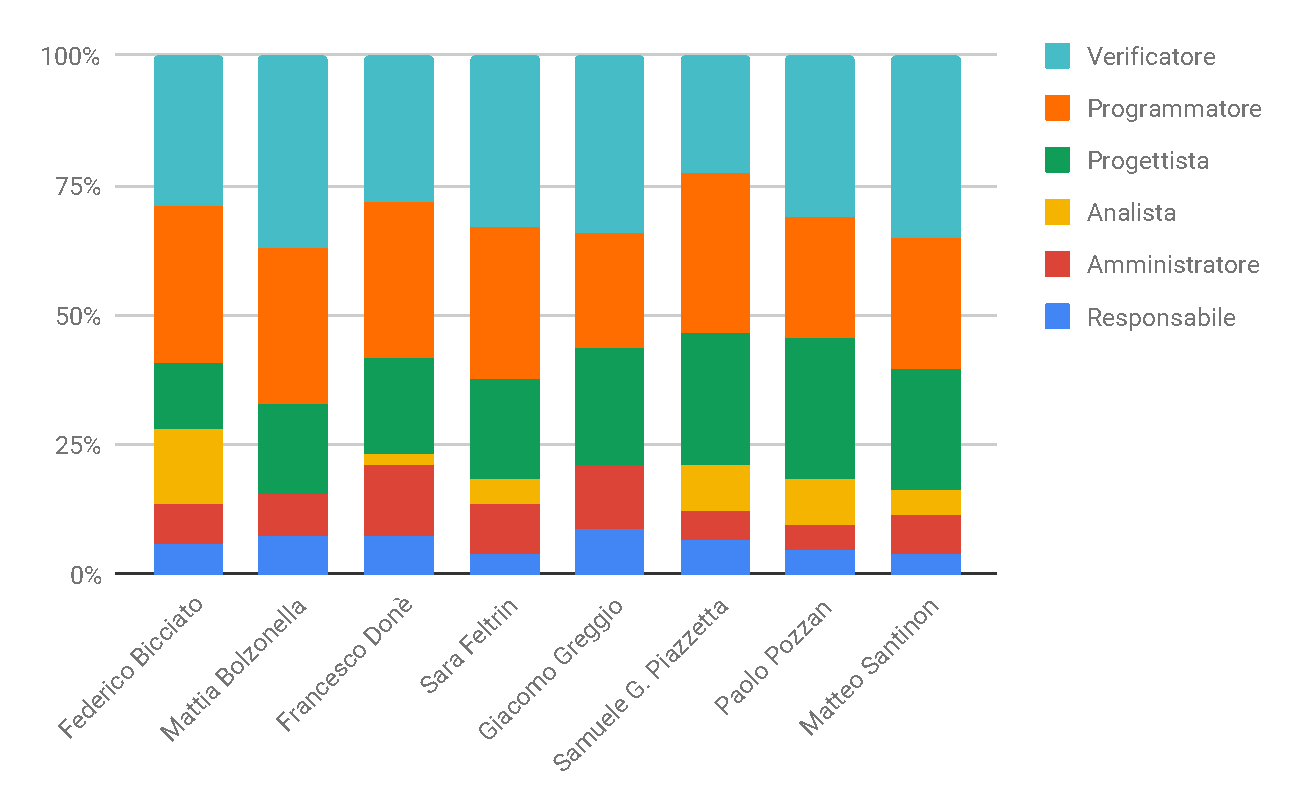
\includegraphics[width=0.9\textwidth]{res/images/istogramma_rendicontate.pdf}\\
				\caption{Istogramma della ripartizione delle ore rendicontate}
			\label{IstogrammaOreRendicontate}
\end{figure}

\paragraph{Prospetto economico}\mbox{}\\
\linebreak
Il totale rendicontato dei costi sostenuti per ogni ruolo è riassunto nella seguente tabella:

\begin{table}[H]
				\centering\renewcommand{\arraystretch}{1.5}
				\arrayrulecolor{white}
                \begin{tabular}{c|c|c}
                               
                \rowcolorhead
                 {\colorhead \textbf{Ruolo}} &
                 {\colorhead \textbf{Ore}} & 
                 {\colorhead \textbf{Costo}} \\
				
                \rowcolorlight
                 {\colorbody Responsabile} & {\colorbody 47} & 
                 {\colorbody \EUR{1.410,00}}  
				\\
				
				\rowcolordark
                 {\colorbody Amministratore} & {\colorbody 46} & 
                 {\colorbody \EUR{920,00}}
				\\	
				
				\rowcolorlight
                 {\colorbody Analista} & {\colorbody 92} & 
                 {\colorbody \EUR{2.300,00}} 
				\\
				
				\rowcolordark
                 {\colorbody Progettista} & {\colorbody 204} & 
                 {\colorbody \EUR{4.488,00}} 
				\\
				
				\rowcolorlight
                 {\colorbody Programmatore} & {\colorbody 127} & 
                 {\colorbody \EUR{1.905,00}} 
				\\
				
				\rowcolordark
                 {\colorbody Verificatore} & {\colorbody 212} & 
                 {\colorbody \EUR{3.180,00}} 
				\\
				
				\rowcolorlight
                 {\colorbody \textbf{Totale}} & {\colorbody 728} & 
                 {\colorbody \EUR{14.203,00}} 
				\\
                

                \end{tabular}
                \caption{Prospetto dei costi delle ore rendicontate}

\end{table}

I dati ottenuti si possono riassumere nel seguente diagramma:
\begin{figure}[H] 
			\centering 
				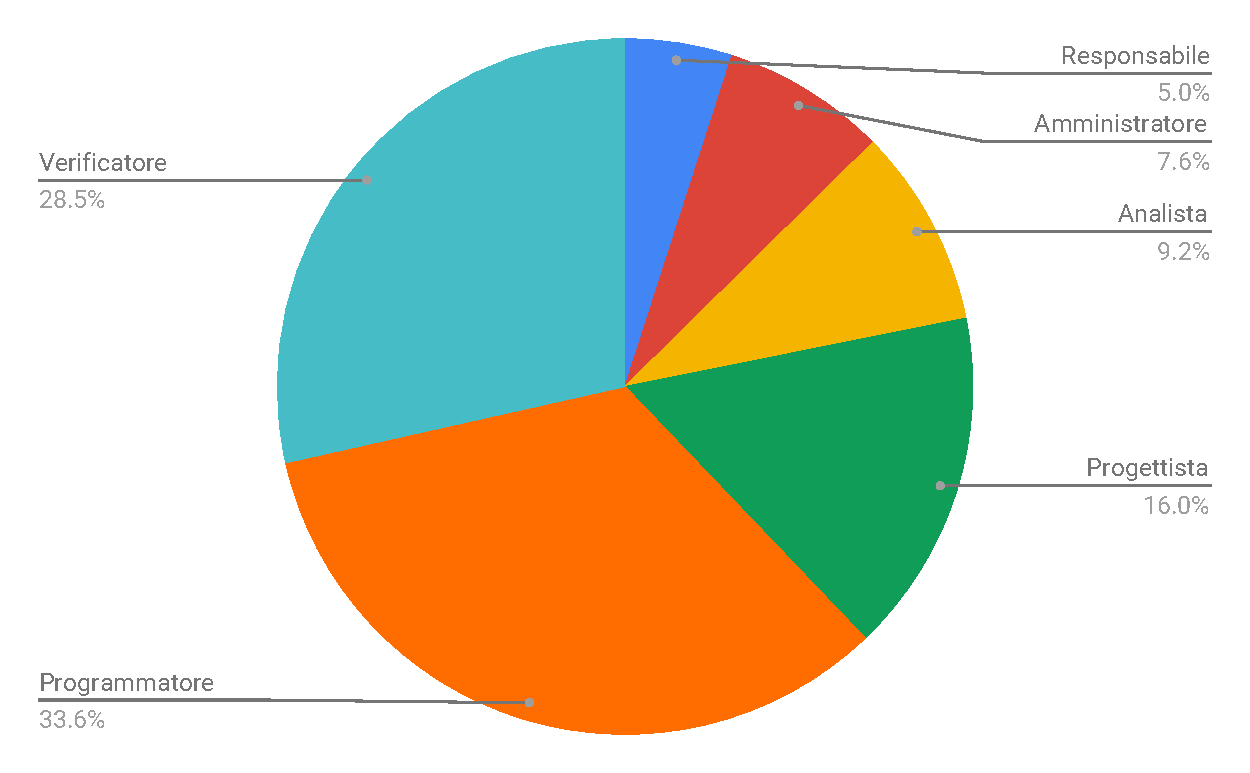
\includegraphics[width=0.7\textwidth]{res/images/areogramma_rendicontate.pdf}\\
				\caption{Areogramma delle ore rendicontate per ruolo}
			\label{AreogrammaOreRendicontate}
\end{figure}

\subsubsection{Conclusioni}
Il costo totale preventivato per il progetto è \EUR{14.203,00}.

